\documentclass{standalone}
%outline around text
\usepackage[outline]{contour}
\contourlength{1.3pt}

%tikz
\usepackage{tikz}
\usetikzlibrary{knots, cd, calc}

\begin{document}




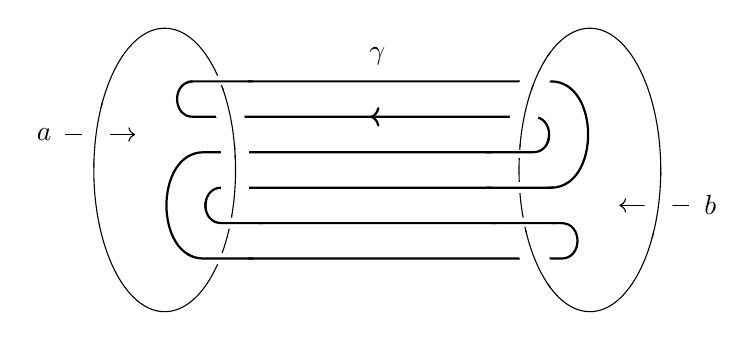
\begin{tikzpicture}[scale=0.9]

\begin{knot}[clip width = 5, ignore endpoint intersections = false,
%draft mode = crossings]
flip crossing/.list = {1, 9, 11, 12, 5, 6, 12}]
\strand (-3, 0) ellipse (1 and 2);
\strand (3, 0) ellipse (1 and 2);

\strand[thick] 
	(-2.6, 1.25) -- 
	(2.45, 1.25) .. controls +(0.7, 0) and +(0.7, 0) ..
	(2.45, -0.25) --
	(-2.2, -0.25) .. controls +(-0.3, 0) and +(-0.3, 0) ..
	(-2.2, -0.75) --
	(2.6, -0.75) .. controls +(0.3, 0) and +(0.3, 0) ..
	(2.6, -1.25) --
	(-2.45, -1.25) .. controls +(-0.7, 0) and +(-0.7, 0) ..
	(-2.45, 0.25) --
	(2.2, 0.25) .. controls +(0.3, 0) and +(0.3, 0) ..
	(2.2, 0.75) --
	(-2.6, 0.75) .. controls +(-0.3, 0) and +(-0.3, 0) ..
	(-2.6, 1.25);

\strand[->] (-4.4, 0.5) -- (-3.4, 0.5);
\strand[->] (4.4, -0.5) -- (3.4, -0.5);
\end{knot}
\draw[thick, ->] (1, 0.75) -- (-0.1, 0.75);
\node at (-4.7, 0.5) {$a$};
\node at (4.7, -0.5) {$b$};
\node at (0, 1.6) {$\gamma$};
\end{tikzpicture}


\end{document}
